
\chapter{Research Methods}
% Implementaatiosta sen verran että tutkimusmetodina on implementoida teknologiaa ja tutkia kuinka se soveltuu arkipäivän käyttöön. Voisi myös miettiä lähestymistä että sulla on ollut kaksi eri tilannetta 1. softa ilman offline"palikkaa/featurea" ja 2. offline palikan kanssa. Tutkit että kuinka offlinepalikka vaikutti sovelluksen käyttökokemukseen.

This chapter introduces the methods followed through this thesis and describes how they are applied on the research.





%% ------------------------------------------
\section{Design Science Research}
% Pyry-viitehox: Pertti Järvinen ja Annikki Järvinen - Tutkimustyön Metodeista (puhelimessa muutama räpsy kyseisestä kirjasta)
% Piirainen-Gonzalez kirja Dropboxista?

% ->avainsana "Konstruktiivinen tutkimus"

This thesis studies the research questions by adapting methodologies and toolbox provided \textit{design science research} (DSR). On the literature this research framework is also referred to \textit{design science} and \textit{design research}.

Hevner and Chatterjee \cite{hevner_design_2010} define design science research as follows:
\begin{quote}
	``Design science research is a research paradigm in which a designer answers questions relevant to human problems via the creation of innovative artifacts, thereby contributing new knowledge to the body of scientific evidence. The designed artifacts are both useful and fundamental in understanding that problem.''
\end{quote}

\begin{figure}
\begin{center}
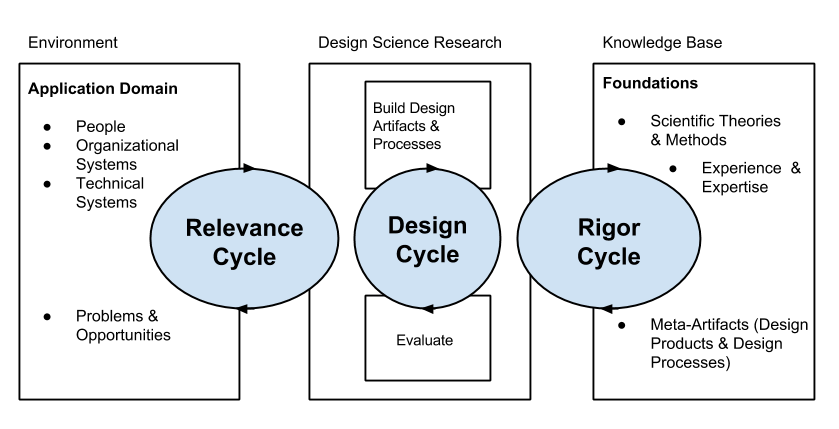
\includegraphics[width=1\textwidth]{assets/dsrcycles.png}
\end{center}
\caption{Design Science Research Cycles, based on the work by Hevner \cite{hevner_three_2007}}
\label{fig:dsrcycles}
\end{figure}


Usually when DSR is applied three related cycles of operations can be recognized, as can be seen in Figure~\ref{fig:dsrcycles} \cite{hevner_three_2007}. First there is the \textit{relevance cycle}, which works as an interface towards the application domain and gathers the information required for producing the artifact. Secondly there is the \textit{rigor cycle}, which provides the existing scientific theories and methods to aid the creation of the artifact. The rigor cycle works both ways, providing feedback on the theories applied on the creation of the artifact and growing up the knowledge base by adding the results to the academic continuum. Finally there is the \textit{design cycle}, where the information from both the application domain and knowledge base meets and possible artifacts for solving the problems found on the application domain are built and evaluated. 

The goal for DSR is that through the three cycles described above, solutions for real-world business problems are found. As a by-product new insights found are increasing the size of the knowledge base via the feedback to the rigor cycle, while the resulting artifacts can be implemented to the application 	domain via feedback to the relevance cycle. \cite{piirainen_constructive_2013}








%% ------------------------------------------
\section{Case Study}

Usually in any research, no matter in which field it is conducted, the size of the sample is directly linked to the quality of the research's outcome. Involving large numbers of participants to the study results in a broader and more representative sample. In some studies research done with a smaller sample will not necessarily be statistically as clear as using a large sample would be. \cite[Page 144]{lazar_research_2010}

Getting a large sample can be extremely challenging or even impossible on some occasions. This should not be a barrier forbidding the conducting of the research, since methods for getting valid results with smaller sample sizes also exists. One of these methods is \textit{case study}, which is also one of the methods applied within this thesis. \cite[Page 144]{lazar_research_2010}

It is also commonly questioned that how valid base does a single case study provide for a scientific generalization. There is no straightforward answer for that. To put it shortly, the aim for case studies should be \textit{``to expand and generalize theories (analytic generalization)''}, not \textit{``to enumerate frequencies (statistical generalization)''}. \cite[Page 15]{yin_case_2013}

On this thesis the research problem is studied in the context of a \textit{single case study} using methods of \textit{design science research}. The possible solutions found and implemented in the case are then evaluated with \textit{semi-structured interviews}.











%% ------------------------------------------
\section{Data Collection with Semi-Structured Interviews}
% "Validating Offline mode User Experience with User Interviews"
% TODO tarttisko tänne jotai tiedelähdetavaraa.....

This section covers the methods on collection of the data about the user experience on the offline support done by conduction series of semi-structured interviews.

As stated in the previous chapters, there is no such thing as an average user of Päikky, due to the fact that users of the system have very different kind of backgrounds. The preparedness for using of technical devices might be very good or it can be almost nonexistent. Because of that one of the goals for this thesis was to study if the offline support implemented is actually understood by the users of Päikky. The received user experience is studied through a series of interviews executed with the nurses using Päikky.

In addition also a interview with the CEO\footnote{Chief Executive Officer} of Päikky was performed. The goal for the CEO's interview was to find out the reasoning and the motives for the offline support development. The amount of available resources and the reason of the allocating them the way which was done is also discussed. The results of the CEO interview are documented thorough this thesis on situations where references to the client organization's decisions can be found and especially in Section~\ref{sec:need-for-offline-support}. Otherwise this section focuses on the interviews done with the kindergarten personnel.

The structure used on the Päikky nurses' interviews can be found from Appendix A. % The structure on the client organization CEO's interview can be found from the appendix B POISTETTU toistaiseksi, ei tuosta liitteestä suurta käytännön hyötyä tulisi



% ###
\subsection{Finding Interviewees}
% Ketä haastateltiin, millä perusteilla valittiin?

Aim for the interviews was to find interviewees whom have used Päikky for an extended period of time, and if possible, also before the production roll-out of the offline support of the system. Other notable factor for the interviewees was the location; it would not been prolific to interview nurses on kindergartens where mobile broadband coverage would not have any issues. On locations where solid Internet connectivity is a given it could be possible that the users would not even have notice the existence of the offline support.

Since Päikky is a product sold explicitly by the client organization, the obvious mean of getting interviewee candidate was to go through them. The client organization provided contact information of two kindergarten managers, whom geographical location had issues with the mobile broadband coverage and the time frame of Päikky's usage would match the requirements set for the interview. These managers were then approached and asked if there would be any volunteers on their staff to take part in a 45 minute interview done on the kindergarten's premises. It was noted to the managers that the optimum interviewee candidate would have used Päikky prior and after the implementation of the offline support, and they would be within the ones who are using Päikky on daily basis.

This process resulted in four interviewees being found, two from each of the kindergartens. 




% ###
\subsection{Preparing Interviews}
% Miten haastattelurunko tehtiin
Prior to the actual execution of the interviews a semi-structured format for the interview was created. The purpose for this structure was to offer an baseline and a general plan for the interview. 

Instead of having a strict, hard-coded script for the interview, the structure was meant to aid the interview process to find out answers and issues that were possibly not realized by the interviewer before actually finding them out during the interview. The questions were meant to set the topic and then allow the interviewer to dig out all the possible aspects from that topic.

% tänne jotai (olemattomasta) testihaastattelusta?






% ###
\subsection{Conducting Interviews}
% "Miten haastattelu toteutettiin"

Four kindergarten nurses were interviewed in total. All of the interviews were conducted face-to-face locally on their kindergarten. 

Every interview started with asking the basic information from the interviewee. Any directly identifying information were not collected. These questions could be considered as a warm-up for the more important topics, but they also were on a key spot providing background information about the interviewee to the interviewer. 

The middle part of the interviews concentrated about how the interviewees used Päikky, and which kind of issues they had faced on it. Every time they described an issue, they were asked how they handled it.

After that the interviewees were asked about their usage of the offline mode on the Kindergarten UI. How often had they experienced the application going into offline mode, how did it change their usage of Päikky, and what kind of issues had they experienced. Also the influence about the limited feature set of offline mode is investigated: did it impede the usage of the application and if so, how.

Also the understanding of the concepts related to the offline mode were enquired: what they considered happening when the device entered the offline mode, how did they understand the under-the-hood events when the device came back from the offline mode. Also the impressions about the location of the data were asked. No direct references were made to the client-server -architecture, but one of the topics aimed to determine if the interviewees had any idea about the master data not being located on their smartphones.

At the end of the interview the interviewees were asked to have a free word on any topic considering Päikky -- the good parts, the bad parts, and the features they wished would exist on Päikky.

Since Finnish was the native language for the interviewer and all the interviewees, the interviews were conducted in that language.

In all the questions were interviewee's usage of Päikky was asked, the question was aimed to be put in the form of ``describe me last time you executed the [action] with Päikky''. This was done trying to get the interviewee to reminisce the actual usage of Päikky, instead of setting them mentally trying to guess what would be the optimal and the instructed way (by the client organization's trainings) of conducting the asked action on Päikky.

During the interview only the interviewer and the interviewee were present. No notes were made during the interview, the situation was aimed to have a relaxed athmosphere, more of a conversation instead of an ``official interview.'' Interviewees were told that if some of the questions seemed too distracting, it would be OK to skip any of them they wish.

All the interviews were recorded.  It was also stated that they would not be identifiable from the results presented on this thesis. After this thesis is finalized, it was promised to the interviewees that the recordings would get destroyed.




% ###
\subsection{Analyzing Interviews}
% "Miten analysointi tehtiin"
% datan keräysmetodina käyttäjä/asiakashaastattelut (muuta?, kehitysdokumentit?)

After the interviews the recordings were listened thoroughly and littered into text. The interview recordings were not exported to the textual format from word for word, but instead key ideas and themes were deducted. Due to the conversational nature of the interviews, word for word littering would not have been beneficial to the research. 

After the major themes for each individual interviewee were found, they were cross-matched in order to find what perspectives were mutual for each of the interview. Also individual interesting viewpoints & opinions were noted on the analyzing process.




